\documentclass[a4paper,10pt,fleqn,twocolumn,twoside,dvipdfmx]{scrartcl}
\usepackage[utf8]{inputenc}
\usepackage[T1]{fontenc}
\usepackage[ngerman]{babel}
\usepackage{microtype}

% \usepackage{mathptmx}
\usepackage{libertine}
\usepackage[libertine,smallerops]{newtxmath}
\addtokomafont{disposition}{\rmfamily}
% \renewcommand\ttdefault{lmtt}
\usepackage[scaled=0.84]{DejaVuSansMono}

\usepackage{amsmath}
\usepackage{amssymb}
\usepackage{booktabs}
\usepackage{listings}
\lstset{basicstyle=\ttfamily\small,commentstyle=\ttfamily}

\usepackage{graphicx}
\usepackage{color}
\definecolor{c1}{RGB}{60,0,40}

\usepackage{geometry}
\geometry{a4paper,left=25mm,right=12mm,top=20mm,bottom=28mm}
\setlength{\columnsep}{6mm}

\numberwithin{equation}{section}

\usepackage[colorlinks=true,linkcolor=black,citecolor=black]{hyperref}
\newcommand{\R}{\mathbb R}
\newcommand{\ee}{\mathrm e}
\newcommand{\unit}[1]{\mathrm{#1}}
\newcommand{\strong}[1]{{\sffamily\bfseries #1}}

\begin{document}

%\thispagestyle{empty}

\noindent
{\huge\textbf{Epidemiologische\\
Grundmodelle}\par}

\tableofcontents

\section{Das klassische SIR-Modell}
\subsection{Modelldefinition}

Die Population von $N$ Individuen wird aufgespalten in die Anteile
$S,I,R$ mit%
\begin{equation}
S+I+R=N.
\end{equation}
Die Ausbreitung der Krankheit verläuft nun gemäß%
\begin{align}
S' &= -\tfrac{1}{N} \beta SI,\\
I' &= \tfrac{1}{N} \beta SI - \gamma I,\\
R' &= \gamma I.
\end{align}
Hierbei handelt es sich um ein autonomes System von gewöhnlichen
Differentialgleichungen für $S(t)$, $I(t)$, $R(t)$.
Wie bei jedem autonomen System ist durch die Gleichungen ein
dynamisches System beschrieben.

Weil dieses Modell noch keine demografische Dynamik enthält,
ist $N$ eine Konstante. Günstig ist daher die Verwendung der
relativen Größen $s:=S/N$, $i:=I/N$, $r:=R/N$. Das System nimmt
damit die Gestalt%
\begin{align}
\label{eq:sir-s} s' &= -\beta si,\\
\label{eq:sir-i} i' &= \beta si - \gamma i,\\
\label{eq:sir-r} r' &= \gamma i
\end{align}
an.

\subsection{Beziehung zur Reproduktionszahl}

Die \emph{effektive Reproduktionszahl} ist definiert gemäß
$R_q := R_0 s$, wobei $R_0$ die \emph{Basisreproduktionszahl} ist.
Hierbei ist $q:=1-s$, so dass man $R_q=R_0$ für $q=0$ erhält. Man nennt
$q$ den immunen Anteil der Population.

Die Reproduktionszahl steht natürlich im Zusammenhang mit dem weiteren
Verlauf der Epidemie. Zur Herleitung fragen wir, unter welchem Umstand
sich die Epidemie bei $i\ne 0$ nicht weiter ausbreitet. Dazu muss
$i'=0$ sein. Eingesetzt in \eqref{eq:sir-i} bedeutet das%
\begin{equation}
0 = (\beta s - \gamma) i \;\Leftrightarrow\; 0 = \beta s - \gamma
\;\Leftrightarrow\; s = \gamma/\beta.
\end{equation}
Nun bedeutet $i'=0$ aber auch $R_q=1$, und daher %
\begin{equation}\label{eq:R0-beta-gamma-from-Rq}
1 = R_q = R_0 s = R_0 \tfrac{\gamma}{\beta}.
\end{equation}
Wir finden die Beziehung
\begin{equation}
\beta = R_0\gamma.
\end{equation}

\subsection{Exponentielle Anfangsphase}

Ist am Anfang der Epidemie $s\approx 1$, verläuft die Ausbreitung
der Krankheit exponentiell. Dies lässt sich leicht einsehen. Setzt
man $s=1$ in \eqref{eq:sir-i} ein, ergibt sich nämlich%
\begin{equation}\label{eq:i-ode-exp}
i' = \lambda i,\quad \lambda := \beta-\gamma.
\end{equation}
Das ist die Dgl. von Exponentialfunktionen, d.\,h. der Lösungen
$i(t) = i(0)\,\ee^{\lambda t}$.

Mathematisch kann man das noch ein wenig genauer herausarbeiten.
Dazu werden die Größen zum Zustandsvektor $x=(s,i,r)$ zusammengefasst.
Das System ist dann abstrakt beschrieben in der Form $x'=f(x)$. Ist
nun $x_0$ eine Ruhelage des dynamischen Systems, genügt die Dynamik
in der Nähe dieser Ruhelage unter gewissen Voraussetzungen
näherungsweise dem linearen System $x' = J_0 x$. Hierbei ist
$J_0:=Df(x_0)$ die Jacobimatrix von $f$ an der Stelle $x_0$.

Eine Ruhelage ist definiert durch $x'(t)=0$ und wird bei den
epidemiologischen Modellen auch als Gleichgewicht (engl.
\emph{equilibrium}) bezeichnet. Dieses kann stabil oder instabil sein.

Der Funktionswert $f(x)$ ist hier die Zusammenfassung der rechten
Seiten der Gleichungen \eqref{eq:sir-s} bis \eqref{eq:sir-r} zu einem
Tupel. Darin darf \eqref{eq:sir-r} entfallen, redundant weil von
den anderen beiden Gleichungen entkoppelt. Das macht%
\begin{equation}
f(\begin{pmatrix}s\\ i\end{pmatrix})
:= \begin{pmatrix}-\beta s i\\ \beta si - \gamma i\end{pmatrix}.
\end{equation}
Somit ergibt sich
\begin{equation}
Df = \begin{pmatrix}
-\beta i & -\beta s\\
\beta i & \beta s - \gamma
\end{pmatrix}.
\end{equation}
Auswertung der Matrix an der Ruhelage $(s,i)=(1,0)$ führt zum linearen
System%
\begin{equation}
\begin{pmatrix}
s'\\ i'
\end{pmatrix}
= \begin{pmatrix}
0 & -\beta\\
0 & \beta-\gamma
\end{pmatrix}
\begin{pmatrix}
s\\ i
\end{pmatrix}.
\end{equation}
Das System enthält \eqref{eq:i-ode-exp} wie gewünscht.

Es gibt noch eine zweite Ruhelage, nämlich $(s,i)=(0,0)$. Die
Auswertung der Matrix bei dieser führt zum System
\begin{equation}
\begin{pmatrix}
s'\\ i'
\end{pmatrix}
= \begin{pmatrix}
0 & 0\\
0 & -\gamma
\end{pmatrix}
\begin{pmatrix}
s\\ i
\end{pmatrix}.
\end{equation}
Demnach verläuft das Abklingen der Epidemie näherungsweise exponentiell
gemäß $i' = -\gamma i$. Zum gleichen Ergebnis gelangt man durch
Einsetzen von $s\approx 0$ in \eqref{eq:sir-i}.

\subsection{Peakhöhe der Infektiösen}

Mit \eqref{eq:sir-i} und \eqref{eq:sir-s} gewinnt man die Dgl.%
\begin{equation}
\frac{\mathrm di}{\mathrm ds} = \frac{i'(t)}{s'(t)}
= \frac{\beta si - \gamma i}{-\beta si} = -1 + \frac{1}{R_0 s},
\end{equation}
deren Lösung
\begin{equation}
i-i_0 = - (s-s_0) + \tfrac{1}{R_0}(\ln s - \ln s_0)
\end{equation}
man durch Separation der Variablen erhält. Umformung dieser
Gleichung liefert%
\begin{equation}\label{eq:const-of-motion}
(i+s)R_0-\ln s = (i_0+s_0)R_0-\ln s_0 = \mathrm{const}.
\end{equation}
D.\,h. die Funktion
\begin{equation}
F(t,(s,i)) := (i+s)R_0 - \ln s
\end{equation}
ist eine erstes Integral der Bewegung. Eine nichtkonstante, stetig
differenzierbare, skalarwertige Funktion $F(t,x)$
heißt \emph{erstes Integral der Bewegung} eines Systems
von Differentialgleichungen erster Ordnung, $x'=f(t,x)$,
wenn $F$ lokal konstant für jede Lösung $x(t)$ ist, d.\,h.
$\tfrac{\mathrm d}{\mathrm dt}F(t,x(t))=0$.

Da hier ein dynamisches System vorliegt, bedeutet dies, dass
das erste Integral der Bewegung auf den
Phasenraum"=Trajektorien $x(t):=(s(t),i(t))$ konstant ist.

Bei $i_\mathrm{max}$ muss $R_q = 1$ sein, also $R_0 s = 1$ bzw.
$s = 1/R_0$. Zur gleichen Einsicht gelangt man natürlich auch
mit der Forderung $\frac{\mathrm di}{\mathrm ds}=0$, deren Lösung auch
$\frac{\mathrm d^2 i}{\mathrm ds^2}<0$ erfüllt. Damit erhalten wir
\begin{equation}
i_\mathrm{max} = i_0 + s_0 - \tfrac{1}{R_0} - \tfrac{1}{R_0}\ln(R_0 s_0)
\end{equation}
aus \eqref{eq:const-of-motion}.

\begin{table}
\begin{tabular}{cll}
\toprule
\strong{Größe} & \strong{Einheit} & \strong{Erklärung}\\
\midrule
$t$ & $\unit{d}$ & Zeit in Tagen\\
$N$ & $\unit{indv}$ & Population\\
$S$ & $\unit{indv}$ & Anfällige, engl. \emph{susceptibles}\\
$E$ & $\unit{indv}$ & Exponierte, engl. \emph{exposed}\\
$I$ & $\unit{indv}$ & Infektiöse, engl. \emph{infectious}\\
$R$ & $\unit{indv}$ & Erholte, engl. \emph{recovered}\\
$\alpha$ & $1/\unit d$ & Kehrwert der Latenzzeit\\
$\beta$ & $1/\unit d$ & Transmissionsrate\\
$\gamma$ & $1/\unit d$ & Erholungsrate\\
$\mu$ & $1/\unit d$ & Sterberate\\
$\nu$ & $1/\unit d$ & Geburtenrate\\
\bottomrule
\end{tabular}
\caption{Größen der Modelle SIR und SEIR.}
\end{table}

\subsection{Ausmaß der Epidemie}

Mit \eqref{eq:sir-s} und \eqref{eq:sir-r} gewinnt man die Dgl.
\begin{equation}\label{eq:ODE-s-r}
\frac{\mathrm ds}{\mathrm dr} = \frac{s'(t)}{r'(t)}
= \frac{-\beta si}{\gamma i} = -R_0 s.
\end{equation}
Diese besitzt die Lösung
\begin{equation}
s = s(r_0)\,\ee^{-R_0 (r-r_0)}.
\end{equation}
Nach Ablauf der Epidemie gilt $i=0$, also $s=1-r$. Man gelangt zu%
\begin{equation}
1-r = s(r_0)\,\ee^{-R_0 (r-r_0)}.
\end{equation}
Dieser Gleichung, \emph{Final size equation} genannt,
kommt eine über das SIR-Modell hinausgehende Bedeutung zu.

Die Gleichung lässt sich in die Form
\begin{equation}
(r-1)R_0\ee^{(r-1)R_0} = -s(r_0)\,R_0\ee^{(r_0-1)R_0}
\end{equation}
bringen, welche von der mathematischen Gestalt $y\ee^y = x$ ist.
Die Anwendung der lambertschen W-Funktion formt diese Gleichung
nach $y$ um, liefert also $y=W(x)$. Demnach erhält man%
\begin{equation}
r = 1+\tfrac{1}{R_0}W(-s(r_0)\,R_0\ee^{(r_0-1)R_0}).
\end{equation}
Unter der Annahme $r_0=0$ und $s(r_0)=1$ hängt $r$ nur von
$R_0$ ab.

Zur praktischen Berechnung des hier relevanten Teils der W-Funktion
betrachtet man das quadratische Taylorpolynom der
Funktion $f(w):=w\ee^w-x$ an der Stelle $-1$ und
bestimmt von diesem die Nullstelle, auf welche noch einmalig die
Fixpunktiteration $w\mapsto x\ee^{-w}$ angewendet
wird. Das Resultat ist
\[w = x\exp(1-\sqrt{2\ee x+2}).\]
Eine gute Näherung der W-Funktion erhält man nun als
\[W(x)\approx \varphi^n(w),\]
wobei $\varphi^n$ die $n$-te Iteration des Newtonverfahrens
\[\varphi(w) = w-\frac{f(w)}{f'(w)} = \frac{x\ee^{-w}+w^2}{w+1}\]
ist. Bereits bei $n=4$ ist der Wert überall in etwa so genau wie
doppelt genaue Fließkommazahlen es erlauben.

\subsection{Infektiöse Zeit}

Der Kehrwert der Erholungsrate $\gamma$ ist interpretierbar
als die mittlere Zeit, die ein Individuum infektiös bleibt. Zur
Untersuchung sei $p(t-t_0)$ die Wahrscheinlichkeit, dass ein zum Zeitpunkt
$t_0$ infiziertes Individuum zum Zeitpunkt $t$ noch infektiös ist.
Hierbei gelte $p(t)=0$ für $t<0$.

Wir würden nun gerne in Erfahrung bringen, welcher Gestalt $p$
denn ist. Dazu schalten wir die Transmission zum Zeitpunkt $t=0$
ab, setzen also ab diesem Zeitpunkt $\beta=0$. Dann gilt einerseits
$i(t)=i(0)p(t)$ und laut \eqref{eq:sir-i} andererseits
$i'=\gamma i$. Einsetzen der Lösung $i(t)=i(0)\ee^{-\gamma t}$
liefert%
\begin{equation}
p(t) = \ee^{-\gamma t}.
\end{equation}
Die Wahrscheinlichkeit zum Zeitpunkt $t$ nicht mehr infektiös zu sein,
$F(t)=1-p(t)$ für $t\ge 0$, ist demnach
die Verteilungsfunktion einer Exponentialverteilung.
Zu dieser gehört die Dichte
$f(t)=\gamma\ee^{-\gamma t}$ und der Erwartungswert
$\mathrm E(X) = 1/\gamma$. In der Tat ist $1/\gamma$ die mittlere
infektiöse Dauer.

Nun drängt sich natürlich die Frage auf, wie sich das Modell so
verallgemeinern lässt, dass $p$ beliebig sein darf.
Unabhängig davon ob $\beta$ konstant ist oder nicht sei
\[(\beta si)(\tau) := \beta(\tau)s(\tau)i(\tau).\]
Zum Zeitpunkt $t$ sind von $i(0)$ noch $i(0)p(t)$ verblieben.
Zu jedem Zeitpunkt $\tau$ kommen $(\beta si)(\tau)$ hinzu,
wovon zum Zeitpunkt $t$ noch $(\beta si)(\tau)p(t-\tau)$ verbleiben.
Das macht%
\begin{equation}\label{eq:int-eq-i}
i(t) = i(0)p(t) + \int_0^t (\beta si)(\tau)p(t-\tau)\,\mathrm d\tau.
\end{equation}
Das Integral kann als Faltung von $\beta si$ und $p$ betrachtet
werden. Die Träger der Funktionen müssen dafür Teilmengen von
$[0,\infty)$ sein, damit das Integrationsintervall äquivalent
von $\R$ auf $[0,t]$ eingeschränkt werden kann.

Aus \eqref{eq:sir-s} erhält man zudem
\begin{equation}\label{eq:int-eq-s}
s(t) = s(0) - \int_0^t (\beta si)(\tau)\,\mathrm d\tau.
\end{equation}
Die Gleichungen \eqref{eq:int-eq-s} und \eqref{eq:int-eq-i}
bilden nun ein nichtlineares System von volterraschen
Integralgleichungen. Zur numerischen
Lösung betrachtet man dieses System als Fixpunktgleichung
$x=\varphi(x)$ mit $x(t)=(s(t),i(t))$. Die Picard"=Iteration
$x_{k+1} = \varphi(x_k)$ sollte dann gegen die Lösung konvergieren.
Als Startfunktion wählt man die konstante Funktion
$x_0(t) := (s_0,i_0)$.

Der geringste Programmieraufwand fällt an, wenn man die Funktionen
bezüglich äquidistanter Stützstellen linear Interpoliert und dabei
für die Integrale übliche Quadraturverfahren heranzieht.

\begin{figure}
\begin{center}
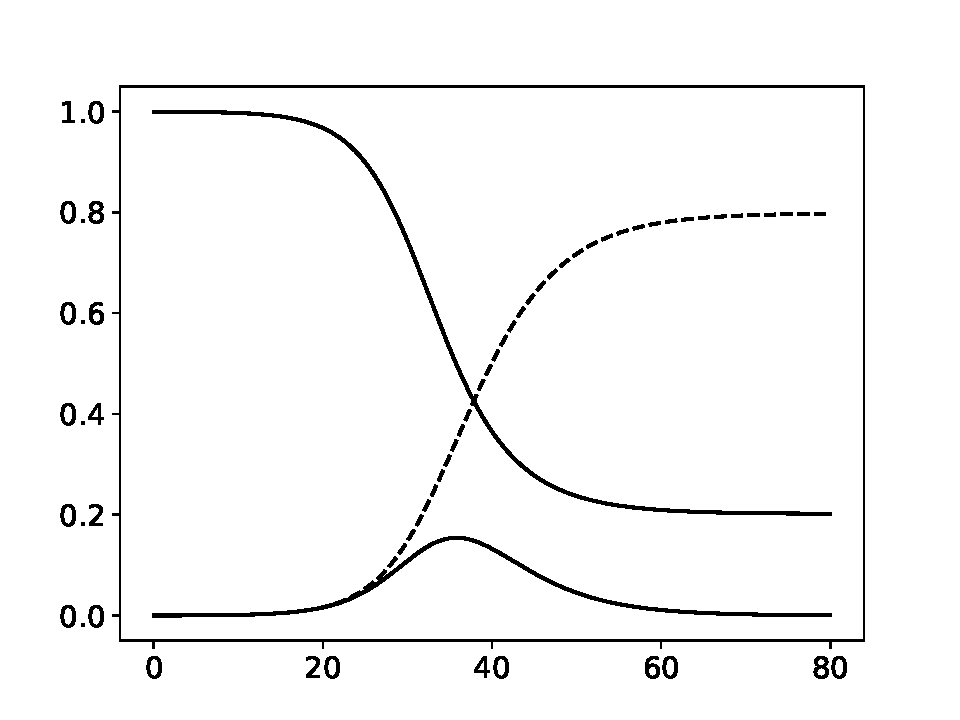
\includegraphics[width=80mm]{img/01-sir.pdf}
Parameter: $R_0 = 2$,\, $\gamma = 1/4$,\, $\beta = R_0\gamma$,\newline
$s_0 = 0$,\, $i_0 = 10000/N$,\, $N = 83200000$.
\end{center}
\caption{Epidemieverlauf im SIR-Modell.}
\end{figure}


\section{Das klassische SEIR-Modell}

\subsection{Modelldefinition}
Die Ausbreitung der Krankheit verläuft gemäß%
\begin{align}
S' &= -\tfrac{1}{N} \beta SI,\\
E' &= \tfrac{1}{N} \beta SI - \alpha E,\\
I' &= \alpha E - \gamma I,\\
R' &= \gamma I.
\end{align}
Umformuliert in relative Größen ist
\begin{align}
\label{eq:seir-s} s' &= - \beta si,\\
\label{eq:seir-e} e' &= \beta si - \alpha e,\\
\label{eq:seir-i} i' &= \alpha e - \gamma i,\\
\label{eq:seir-r} r' &= \gamma i.
\end{align}

\subsection{Beziehung zur Reproduktionszahl}

Damit $R_q=1$ gilt, muss $e'=0$ und $i'=0$ sein. Eingesetzt in
\eqref{eq:seir-e} und \eqref{eq:seir-i} bringt das $\alpha e=\beta si$
und $\alpha e = \gamma i$. Somit ist $\beta s = \gamma$. Wie
bei \eqref{eq:R0-beta-gamma-from-Rq} ergibt sich
\begin{equation}
\beta = R_0\gamma.
\end{equation}

\subsection{Ausmaß der Epidemie}

Die Dgl. \eqref{eq:ODE-s-r} und der weitere Abschnitt
einschließlich der Final size equation sind weiterhin gültig.
Nach Ablauf der Epidemie gilt neben $i=0$ nun zusätzlich $e=0$.

\subsection{Exponentielle Anfangsphase}

Am Anfang der Epidemie kann man wie beim SIR"=Modell $s\approx 1$ setzen
bzw. die Linearisierung mit der Jacobimatrix $Df(x_0)$ betrachten.
Beide Ansätze führen zum linearen System
\begin{equation}\label{eq:ei-linear}
\begin{pmatrix}e'\\ i'
\end{pmatrix}
= A\begin{pmatrix}
e\\ i
\end{pmatrix}
= \begin{pmatrix}
-\alpha & \beta\\
\alpha & -\gamma
\end{pmatrix}
\begin{pmatrix}
e\\ i
\end{pmatrix}.
\end{equation}
Für die Eigenwerte der Matrix gilt
\begin{equation}\label{eq:ei-eigenvalue}
0 = \det(A-\lambda E_2) = (\alpha+\lambda)(\gamma+\lambda)-\alpha\beta.
\end{equation}
Für $R_0>1$ sind das unter normalen Umständen zwei Eigenwerte,
einer positiv, der andere negativ. Demnach ist die Ruhelage
vom Typ Sattelpunkt und somit instabil, wie zu erwarten war.
Für $R_0<1$ sind es zwei negative Eigenwerte, die Ruhelage daher
asymptotisch stabil und vom Typ uneigentlicher Knoten.

Der Ansatz $i=i(0)\ee^{\lambda t}$ ist zielführend und
ergibt $e=\tfrac{1}{\alpha}(\gamma+\lambda)i$. Ferner lässt sich
zeigen, dass die Wachstumskonstante $\lambda$ der Eigenwert
aus \eqref{eq:ei-eigenvalue} ist. Einerseits muss das aus
\eqref{eq:ei-linear} hervorgehen. Alternativ benutzt man $i'=\lambda i$,
womit %
\[1-s = e + i + r
= \tfrac{\gamma+\lambda}{\alpha}i + i + \tfrac{\gamma}{\lambda} i
= (\tfrac{\gamma+\lambda}{\alpha} + 1 + \tfrac{\gamma}{\lambda})i\]
ist. Leitet man diese Gleichung nun auf beiden Seiten ab,
benutzt $-s' = \beta si$ und dividiert anschließend durch $i$,
kommt man auf%
\begin{equation}
\beta s = (\tfrac{\gamma+\lambda}{\alpha} + 1 + \tfrac{\gamma}{\lambda})\lambda.
\end{equation}
Mit $s\approx 1$ ergibt sich daraus \eqref{eq:ei-eigenvalue}.

Somit ist eine Beziehung zwischen $\lambda$ und den Parametern
$\alpha,\beta,\gamma$ gewonnen.

\section{SIR-Modell mit Demografie}
\subsection{Modelldefinition}
Angenommen, es gibt eine Geburtenrate $\nu$ (lat.-engl. \emph{natality rate}), 
und eine Sterberate $\mu$ (lat.-engl. \emph{mortality rate}). Zur Änderung der
Anfälligen kommen dann $\nu N$ hinzu, wobei $N$ die aktuelle
Bevölkerungszahl ist. Von jeder Gruppe $X$ versterben außerdem $\mu X$.

Die Ausbreitung verläuft demnach gemäß%
\begin{align}
S' &= \nu N - \tfrac{1}{N}\beta SI - \mu S,\\
I' &= \tfrac{1}{N}\beta SI - \gamma I - \mu I,\\
R' &= \gamma I - \mu R.
\end{align}
Zu beachten ist, dass $N=S+I+R$ nun keine Konstante mehr
ist. Aus den Dgln. ergibt sich allerdings
\begin{equation}\label{eq:ODE-N}
\begin{split}
N' &= S'+I'+R' = \nu N - \mu S - \mu I - \mu R\\
&= \nu N - \mu N = (\nu-\mu)N.
\end{split}
\end{equation}
Bei der Umrechnung in die relativen Größen ist nun bei der
Ableitung jeweils die Produktregel anzuwenden, also
\[S' = (Ns)' = N's + Ns'\]
usw. Das führt mit \eqref{eq:ODE-N} zum System
\begin{align}
s' &= \nu - \beta si - \nu s,\\
i' &= \beta si - \gamma i - \nu i,\\
r' &= \gamma i - \nu r.
\end{align}
Verblüffend ergibt sich das gleiche System, als wäre
$N$ konstant mit $\nu = \mu$. Es genügt daher ohne Beschränkung
der Allgemeinheit die Betrachtung dieses Falls.

\newpage
\section{Berechnung}

\begin{figure}[h!]
\begin{lstlisting}[language=Python]
from numpy import array as vector

# Explizites Euler-Verfahren
def euler_method(f,t0,x0,t1,h):
    t = t0; x = x0
    a = [[t,x]]
    for k in range(0,1+int((t1-t0)/h)):
        t = t0 + k*h
        x = x + h*f(t,x)
        a.append([t,x])
    return a

def sir_model(beta,gamma):
    def f(t,x):
        s,i,r = x
        return vector([
            -beta*s*i,
            beta*s*i - gamma*i,
            gamma*i
        ])
    return f

def sir_simulation(beta,gamma,i0,days,step=0.1):
    x0 = vector([1.0-i0,i0,0.0])
    model = sir_model(beta,gamma)
    return euler_method(model,0,x0,days,step)

def diagram(simulation):
    import matplotlib.pyplot as plot
    figure,axes = plot.subplots()
    t,x = zip(*simulation())
    s,i,r = zip(*x)
    axes.plot(t,s, color = "#000000")
    axes.plot(t,i, color = "#000000")
    axes.plot(t,r, color = "#000000",
        linestyle = '--')
    plot.show()

# N: Einwohnerzahl von Deutschland 2019/2020
def simulation1():
    R0 = 2.0; gamma = 1/4.0; N = 83200000
    return sir_simulation(
        beta = R0*gamma, gamma = gamma,
        i0 = 10000.0/N, days = 80)

diagram(simulation1)
\end{lstlisting}
\caption{Simulation mittels SIR-Modell}
\end{figure}


\mbox{}
\vfill

\noindent
{\small Dieser Text steht unter der Lizenz\\
Creative Commons CC0.}

\end{document}
